\documentclass[conference]{IEEEtran}
\usepackage[T1]{fontenc}
\usepackage[utf8]{inputenc}
\usepackage{lmodern}
\usepackage{amsmath,amssymb,url,graphicx}
\newcommand{\T}{\mathsf{T}}
\newcommand{\TL}{\mathsf{TL_{struct}}}
\newcommand{\TLV}{\mathsf{TLV}}

\title{ECM-TQAG: An Evidence-First Protocol for Traceable Multimodal Textbook Question Construction}
\author{\IEEEauthorblockN{Xuan Van Mai\IEEEauthorrefmark{1}, Van Long Tran\IEEEauthorrefmark{1}, Viet Long Tran\IEEEauthorrefmark{2}, Van Khang Nguyen\IEEEauthorrefmark{1}, and Tuong Tri Nguyen\IEEEauthorrefmark{1},\IEEEauthorrefmark{3}}\IEEEauthorblockA{\IEEEauthorrefmark{1}University of Education, Hue University, Hue, Vietnam}\IEEEauthorblockA{\IEEEauthorrefmark{2}University of Law, Hue University, Hue, Vietnam}\IEEEauthorblockA{\IEEEauthorrefmark{3}Institute of Open Education and Information Technology, Hue University, Hue, Vietnam}}

\begin{document}
\maketitle
\begin{abstract}
ECM-TQAG is an evidence-first protocol for constructing traceable multimodal textbook question-answering items. It compares direct, answer-first, and evidence-chain generation from fixed text--structure--image packages. In the evidence-chain method, a planner proposes a source-bound document graph and requests a motif from a closed catalog. Deterministic code validates and matches the motif, compiles it into a restricted program, executes that program, and derives answer atoms with node, edge, and program-step provenance. A separate realizer receives the locked construction and produces one four-option question. We instantiate the protocol on 16 OCR-derived chunks from 9 Vietnamese law textbooks, forming a $16\times3\times3=144$-cell matrix, and generate every cell with an open-weight vision--language model. Mechanical replay confirms executable structural and provenance validity: 143 of 144 records parse into the required schema, all retained records satisfy option distinctness and answer-index range, and the single rejection is a genuine generator fault caught by the checker. Two independent judges from different model families then score every record on a four-dimension rubric under choice permutation and condition blinding; agreement is moderate ($\mathrm{QWK}$ 0.37--0.69), so the scores are reported as descriptive agreement rather than semantic or legal validity. Under Friedman tests over complete chunk blocks, neither construction method nor evidence condition separates on faithfulness, answerability, or distractor quality; only question depth shows a method effect, and its post-hoc contrasts do not survive Holm correction. We report these null results explicitly and identify rubric refinement and depth-oriented prompting as the operative next steps.
\end{abstract}
\begin{IEEEkeywords}
multimodal question generation, textbook question answering, evidence-grounded generation, provenance-aware generation, document understanding
\end{IEEEkeywords}

\section{Introduction}
Textbooks distribute instructional content across prose, headings, tables, diagrams, charts, and page layout. A multimodal textbook question-answering (TQA) item therefore benefits from an inspectable relation among its answer, supporting evidence, and visual or structural context. Document models combine text, geometry, and visual representations \cite{xu2020layoutlm,xu2021layoutlmv2,huang2022layoutlmv3}; document, table, and chart QA demonstrate the role of structured and visual evidence \cite{mathew2021docvqa,herzig2020tapas,tito2023multipage,kafle2018dvqa,masry2022chartqa}; and question generation supports visual and educational authoring \cite{mostafazadeh2016generating,zhu2016visual7w,heilman2010good,kurdi2020systematic}. This motivates a construction pipeline that preserves answer provenance before question formulation and records the evidence modalities used.

This work addresses traceable multimodal TQA construction from OCR-derived textbook chunks. The primary system output is one ECM-TQAG multimodal TQA item; the nine combinations used in the experiment are evaluation conditions, not nine independent products of the proposed method. ECM-TQAG adopts an evidence-first, answer-before-question sequence:
\begin{equation}
G_m \rightarrow z \rightarrow (A,\Gamma) \rightarrow q \rightarrow \mathcal{C},
\end{equation}
where a matched motif $G_m$ supplies a restricted program $z$, yielding typed answer atoms $A$ and a provenance trace $\Gamma$ before a four-option question $q$ is checked by $\mathcal{C}$. The matcher, compiler, executor, and tracer compute $G_m$, $z$, $A$, and $\Gamma$ through deterministic local code. The approach combines compositional reasoning over scenes, diagrams, and structured visual evidence \cite{johnson2017clevr,hudson2019gqa,kafle2018dvqa,masry2022chartqa} with provenance models that distinguish source records from derived artifacts \cite{moreau2013prov}.

The contributions are: (i) a source-grounded representation that begins with OCR text and retains aligned layout and visual context when available; (ii) motif-guided, answer-before-question derivation of atoms and traces, in which motif matching, program compilation, execution, and tracing are executable rather than declarative; (iii) a replayable validation path for derivation, atom--trace correspondence, and MCQ consistency; and (iv) an empirical evaluation across evidence conditions and construction methods.

\section{ECM-TQAG Construction Protocol}
\begin{figure*}[t]
\centering
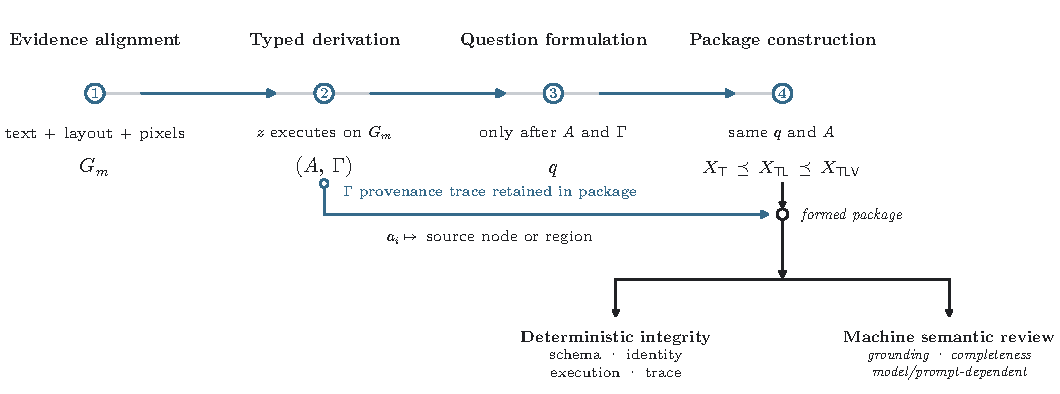
\includegraphics[width=\textwidth]{ecm_tqag_architecture.pdf}
\caption{ECM-TQAG construction and experimental evaluation. A user supplies OCR text from a textbook PDF and selects an LLM runtime or API provider. The proposed ECM-TQAG path constructs one multimodal TQA item with four choices, evidence references, and a provenance trace. For comparison, the evaluation instantiates a nine-cell matrix from three evidence views (text, text plus layout, and text plus visual context) crossed with Direct, Answer-first, and ECM-TQAG construction; these scenarios support evaluation rather than define the primary output.}
\label{fig:architecture}
\end{figure*}
\subsection{Input and multimodal evidence representation}
The user-facing input is an OCR-derived chunk from a textbook PDF. The chunk supplies extracted text and may retain source location metadata; the system associates structural/layout cues and the corresponding page visual when the selected experimental condition permits them. We represent the available evidence as $D=(T,L,V,M,\Pi)$: text, structure/layout, visual regions, metadata, and source-level provenance. Parsing and alignment produce
\begin{equation}
G=(N,E,\rho),\qquad N=N_T\cup N_L\cup N_V\cup N_M,
\end{equation}
where $\rho:N\rightarrow\Pi$ links each node to a source descriptor such as page, region, character span, and extraction metadata. This source mapping is distinct from the item-level trace $\Gamma$ \cite{moreau2013prov}. The mapping is recomputed deterministically from the supplied chunk and aligned evidence, so every answer atom can be related back to the source material used for construction.

For each selected chunk, let $c\in K=\{\T,\TL,\TLV\}$ denote an evidence-condition label. ECM-TQAG forms the paired evidence packages
\begin{equation}
\mathcal{X}_{\T}=(T),\quad \mathcal{X}_{\TL}=(T,L),\quad \mathcal{X}_{\TLV}=(T,L,V).
\end{equation}
The three conditions are used only to measure the contribution of additional evidence during the experiment: text-only, text plus layout, and text plus visual context. The proposed ECM-TQAG output is produced by the evidence-first construction path and records the evidence condition used for that item.

\subsection{Evidence-first construction of the ECM-TQAG item}
The construction follows one spine:
\begin{equation}
\text{OCR chunk} \rightarrow G \rightarrow G_m \rightarrow z \rightarrow (A,\Gamma) \rightarrow q \rightarrow \mathcal{C}.
\end{equation}
The language model proposes a typed evidence graph $G$ and a motif request from the supplied multimodal evidence. A motif template defines the admissible pattern and derivation template. A matched $G_m\subseteq G$ supplies the restricted program $z$; unresolved inputs or incomplete provenance terminate construction. The matcher checks that the requested roles and relations are supported by the source-bound graph rather than accepting a model-supplied label alone.

A deterministic compiler maps the successful match to a restricted program $z$ over typed values. Execution yields an answer structure and a trace:
\begin{equation}
A=\mathrm{Exec}(z,G_m),\qquad \Gamma=\mathrm{Trace}(z,G_m).
\end{equation}
Here $A=(a_1,\dots,a_k)$ contains answer atoms and $\Gamma=(\gamma_1,\dots,\gamma_k)$ links each $a_j$ to source nodes or regions via $\rho$. A question realizer then receives the locked answer construction and produces one four-option multimodal TQA item. It must preserve the answer atoms, evidence anchors, and executor-derived answer selection. Thus the answer is fixed before wording the question, while the final record contains the question, choices, selected answer, multimodal evidence references, and provenance trace. For ECM--$\TLV$, the matched construction must bind a visual node, providing the formal visual-evidence condition used in the evaluation \cite{goyal2017making,agrawal2018don}.

\subsection{Validation and replay}
The final check set $\mathcal{C}$ enforces a well-formed derivation, non-empty answer atoms, atom--trace correspondence, four distinct options, and answer--choice agreement. Replay recomputes the source mapping, motif match, restricted program, answer atoms, and provenance trace from the supplied evidence. A failed construction is retained as rejected rather than silently converted into a valid TQA item. These checks establish structural and provenance validity; semantic correctness, legal correctness, pedagogical quality, and visual dependence require separate assessment.

\subsection{Direct and answer-first baselines}
\emph{Direct} requests one four-option MCQ from a directly supported proposition. \emph{Answer-first} requires a declared answer and evidence excerpt before the question and same-domain distractors; a deterministic check requires the declared answer to equal the selected option. Both retain source-labelled evidence anchors. ECM-TQAG adds typed graph matching, restricted execution, answer atoms, and program traces, so the chunk and available evidence remain fixed while the construction protocol changes.

\section{Experimental Evaluation}
\label{sec:experiments}
We evaluate 16 screened chunks drawn from 9 Vietnamese law textbooks under a full
factorial design with three evidence conditions and three construction methods,
yielding $16\times3\times3=144$ cells. The conditions isolate the contribution of
evidence modalities: $\T$ supplies extracted text; $\TL$ adds declared document
structure; and $\TLV$ adds the attached page image. Chunk screening, image--page
verification, and package construction are recorded in a versioned manifest
(48 evidence packages, 18 verified page images, SHA-256 digest per package), and
every request is keyed to that digest so a cell can be replayed against the exact
evidence it consumed.

\begin{table}[t]
\centering
\caption{Evaluation design and request allocation.}
\label{tab:design}
\small
\resizebox{\columnwidth}{!}{%
\begin{tabular}{lcc}
\hline
Factor & Levels & Cells/requests \\
\hline
Source contexts & 16 chunks from 9 textbooks & 16 \\
Evidence & $\T$, $\TL$, $\TLV$ & 3 \\
Method & Direct, Answer-first, ECM-TQAG & 3 \\
Full factorial matrix & $16\times3\times3$ & 144 cells \\
Evidence packages & 16 chunks $\times$ 3 conditions & 48 \\
Verified page images & aligned to $\TLV$ packages & 18 \\
\hline
\end{tabular}
}%
\end{table}

\subsection{Models and separation of roles}
Generation and assessment use disjoint model families to avoid same-family
self-preference. All 144 cells are generated by \texttt{qwen3-vl-32b-instruct}
(temperature $0$, fixed seed). Assessment uses two independent judges from two
other families: \texttt{claude-sonnet-5} and \texttt{gpt-5.6-terra}. Judges never
observe the method label, the evidence condition, the generator identity, or the
run identifier; option order is permuted per item under a fixed seed and the gold
index is remapped accordingly, so position priors cannot be exploited. Each judge
returns integer scores in $[1,5]$ on four dimensions: faithfulness to the supplied
evidence, answerability from that evidence alone, distractor quality, and
reasoning depth.

\subsection{Mechanical validity of the generated records}
The mechanical audit is deterministic and independent of any judge. Of 144 cells,
143 (99.3\%) satisfied the record contract and one was rejected because the
realizer emitted a single option instead of four. Across the 143 accepted records,
the answer index was in range in 100.0\% of cells and the four options were
mutually distinct in 100.0\% of cells, while the declared answer string matched the
selected option in 89.6\% of cells. Literal grounding was measured by matching the
declared evidence excerpt against the supplied source: 43.8\% of excerpts were
exact substrings of the source, whereas 96.5\% of excerpt 5-grams were present in
the source. The gap between these two figures is the central grounding finding:
the generator paraphrases while quoting, so excerpt fields are near-verbatim rather
than verbatim, and an exact-match gate alone would misclassify most records.

A second generator from a different family (\texttt{claude-sonnet-4.6}) was run on
the identical 144-cell design as a reference point. It reached 144/144 contract
compliance, 97.9\% answer--option agreement, and 79.2\% exact-substring excerpts
against 98.9\% 5-gram coverage. The two generators therefore differ in quoting
discipline by a wide margin (43.8\% versus 79.2\% verbatim) while agreeing closely
on 5-gram coverage (96.5\% versus 98.9\%), which indicates that near-verbatim
grounding is stable across families but literal quoting is model-specific.

\subsection{Judge agreement}
Both judges scored 142 of the 143 accepted cells; one cell was lost because a
judge response was truncated mid-JSON. Table~\ref{tab:agreement} reports agreement
on these 142 common cells. Exact agreement is high on faithfulness and
answerability (0.901 and 0.894) and much lower on distractor quality and depth
(0.549 and 0.585), yet agreement within one scale point exceeds 0.95 on all four
dimensions. Quadratic-weighted $\kappa$ ranges from 0.369 to 0.686. Under
conventional thresholds this is moderate agreement, substantial only for
answerability. The pattern indicates that the two judges order items consistently
but apply different strictness on the two more subjective dimensions, so
distractor quality and depth are reported as descriptive indicators rather than as
calibrated measurements.

\begin{table}[t]
\centering
\caption{Cross-judge agreement on 142 commonly scored cells
(\texttt{claude-sonnet-5} versus \texttt{gpt-5.6-terra}).}
\label{tab:agreement}
\small
\begin{tabular}{lcccc}
\hline
Dimension & Exact & Within 1 & QWK & $r$ \\
\hline
Faithfulness & 0.901 & 0.965 & 0.466 & 0.592 \\
Answerability & 0.894 & 0.958 & 0.686 & 0.693 \\
Distractor quality & 0.549 & 0.979 & 0.369 & 0.401 \\
Reasoning depth & 0.585 & 0.986 & 0.416 & 0.550 \\
\hline
\end{tabular}
\end{table}

\subsection{Method and condition comparison}
Judge scores are averaged over the two judges, then averaged within each
(chunk, factor level) block, giving one paired observation per chunk. Fourteen of
the 16 chunks yielded a complete $3\times3$ block and form the analysis set. Each
factor is tested with a Friedman test over the three levels, followed by
Wilcoxon signed-rank post-hoc tests with Holm correction, Cliff's $\delta$, and
bootstrap 95\% confidence intervals for the median paired difference
($10^4$ resamples, fixed seed).

\begin{table}[t]
\centering
\caption{Method comparison over 14 complete chunk blocks. Values are block means
of judge-averaged scores; $p$ from the Friedman test; $W$ is Kendall's $W$.}
\label{tab:method}
\small
\resizebox{\columnwidth}{!}{%
\begin{tabular}{lccccc}
\hline
Dimension & Direct & Answer-first & ECM & $p$ & $W$ \\
\hline
Faithfulness & 4.821 & 4.821 & 4.893 & 0.261 & 0.096 \\
Answerability & 4.798 & 4.726 & 4.690 & 0.661 & 0.030 \\
Distractor quality & 3.345 & 3.262 & 3.321 & 0.829 & 0.013 \\
Reasoning depth & 1.381 & 1.405 & 1.571 & 0.024 & 0.266 \\
Composite & 3.586 & 3.554 & 3.619 & 0.571 & 0.040 \\
\hline
\end{tabular}
}%
\end{table}

Table~\ref{tab:method} shows no significant method effect on faithfulness,
answerability, distractor quality, or the composite score. Reasoning depth is the
only dimension with a significant Friedman result ($\chi^2=7.43$, $p=0.024$,
$W=0.266$), with ECM-TQAG highest in block mean (1.571 versus 1.381 for direct and
1.405 for answer-first). However, no pairwise contrast survives Holm correction:
direct versus ECM gives $p_{\text{raw}}=0.064$, $p_{\text{holm}}=0.160$,
$\delta=-0.276$, and a bootstrap interval $[-0.333,0.000]$ that includes zero;
answer-first versus ECM gives $p_{\text{raw}}=0.053$, $p_{\text{holm}}=0.160$,
$\delta=-0.240$, with the same interval behaviour. We therefore report a
consistent directional advantage for ECM-TQAG on reasoning depth that this sample
does not establish as a pairwise difference.

\begin{table}[t]
\centering
\caption{Evidence-condition comparison over the same 14 complete chunk blocks.}
\label{tab:condition}
\small
\resizebox{\columnwidth}{!}{%
\begin{tabular}{lccccc}
\hline
Dimension & $\T$ & $\TL$ & $\TLV$ & $p$ & $W$ \\
\hline
Faithfulness & 4.905 & 4.952 & 4.679 & 0.174 & 0.125 \\
Answerability & 4.762 & 4.905 & 4.548 & 0.356 & 0.074 \\
Distractor quality & 3.286 & 3.333 & 3.310 & 0.819 & 0.014 \\
Reasoning depth & 1.488 & 1.464 & 1.405 & 0.282 & 0.090 \\
Composite & 3.610 & 3.664 & 3.485 & 0.361 & 0.073 \\
\hline
\end{tabular}
}%
\end{table}

No evidence condition shows a significant effect (Table~\ref{tab:condition}); all
Friedman $p$-values exceed 0.17 and every Kendall's $W$ is below 0.13. Adding the
page image did not raise judged quality on any dimension, and $\TLV$ has the lowest
block mean on faithfulness, answerability, and the composite. This is a negative
result about the current visual pathway rather than evidence that page images are
uninformative: the audit confirms image--page alignment, so the more likely
explanation is that the realizer does not convert an attached page visual into
additional judged quality under the present prompts.

Across dimensions, the absolute score levels are as informative as the contrasts.
Faithfulness and answerability sit near the top of the scale (block means
$4.69$--$4.95$), whereas reasoning depth sits near the bottom
($1.41$--$1.57$). The generated items are thus well grounded and answerable from
the supplied evidence but predominantly retrieval-level, which both judges noted
independently in their free-text comments. Raising item depth, not grounding, is
the binding constraint on this pipeline.

\section{Limitations}
Five limitations bound these results. First, the analysis set is 14 complete chunk
blocks from 9 textbooks; this pilot scale yields low power, so the absence of
significant effects on most dimensions cannot be read as evidence of equivalence.
Second, all quality scores are model-based. Two judges from families disjoint from
the generator establish descriptive agreement, not semantic or legal validity; no
human or expert anchor is included in this study, and the moderate
quadratic-weighted $\kappa$ on distractor quality (0.369) and depth (0.416) marks
those two dimensions as the least calibrated. Third, the rubric applies a single
integer scale per dimension and does not separate legal correctness from general
factual correctness, which a domain expert review would need to disentangle.
Fourth, literal grounding is measured against the supplied OCR text, so a
near-verbatim excerpt scores highly on 5-gram coverage even when it is not an exact
quotation; the 43.8\% versus 96.5\% gap quantifies this and should be read as a
property of the measurement as well as of the generator. Fifth, the negative
$\TLV$ result is specific to the prompts, the single vision-language generator, and
the page-level image granularity used here; region-level visual evidence or a
different realizer could change it. Distractor quality, pedagogical usefulness, and
image dependence remain contingent on documented expert review and
learner-oriented studies \cite{kurdi2020systematic,haladyna2002review,goyal2017making,agrawal2018don}.

\section{Conclusion}
ECM-TQAG provides an executable evidence-first protocol for multimodal textbook MCQ construction. Its planner proposes a source-bound document graph; local code matches a closed-catalog motif, compiles and executes a restricted program, and derives provenance-bearing answer atoms; and its isolated realizer receives only that sealed construction. The method makes structural construction replayable while keeping stronger claims about graph semantics, legal correctness, pedagogy, and visual necessity contingent on completed expert evaluation.

\section*{Acknowledgment}
The authors thank the Institute of Open Education and Information Technology, Hue University, for providing research data and a laboratory environment for this study.

\section*{Funding}
This work was supported by project DHH2026.

\section*{Data, Code, and Materials Availability}
Code, tests, and synthetic fixtures are available at \url{https://github.com/mxuanvan02/TQA_Pipeline}. Access to source textbooks, page images, and detailed model records follows the applicable permissions and rights review; derivative release materials are provided through the documented release channel.

\section*{Conflict of Interest}
The authors declare no competing interests.

\section*{Generative-AI Use Disclosure}
Generative-AI tools were used to assist with grammar editing, code development, and figure preparation.

\bibliographystyle{IEEEtran}
\bibliography{references}
\end{document}
